\documentclass[a4paper]{article}
\usepackage[utf8]{inputenc}
\usepackage{amsmath}
\usepackage{amssymb}
\usepackage{caption}
\usepackage{mathtools}
\usepackage{amsfonts}
\usepackage{lastpage}
\usepackage{tikz}
\usepackage{float}
\usepackage{textcomp}
\usetikzlibrary{patterns}
\usepackage{pdfpages}
\usepackage{gauss}
\usepackage{fancyvrb}
\usepackage[table]{colortbl}
\usepackage{fancyhdr}
\usepackage{graphicx}
\usepackage[margin=2.5 cm]{geometry}

\definecolor{listinggray}{gray}{0.9}
\usepackage{listings}
\lstset{
	language=,
	literate=
		{æ}{{\ae}}1
		{ø}{{\o}}1
		{å}{{\aa}}1
		{Æ}{{\AE}}1
		{Ø}{{\O}}1
		{Å}{{\AA}}1,
	backgroundcolor=\color{listinggray},
	tabsize=3,
	rulecolor=,
	basicstyle=\scriptsize,
	upquote=true,
	aboveskip={0.2\baselineskip},
	columns=fixed,
	showstringspaces=false,
	extendedchars=true,
	breaklines=true,
	prebreak =\raisebox{0ex}[0ex][0ex]{\ensuremath{\hookleftarrow}},
	frame=single,
	showtabs=false,
	showspaces=false,
	showlines=true,
	showstringspaces=false,
	identifierstyle=\ttfamily,
	keywordstyle=\color[rgb]{0,0,1},
	commentstyle=\color[rgb]{0.133,0.545,0.133},
	stringstyle=\color[rgb]{0.627,0.126,0.941},
  moredelim=**[is][\color{blue}]{@}{@},
}

\lstdefinestyle{base}{
  emptylines=1,
  breaklines=true,
  basicstyle=\ttfamily\color{black},
}

\pagestyle{fancy}
\def\checkmark{\tikz\fill[scale=0.4](0,.35) -- (.25,0) -- (1,.7) -- (.25,.15) -- cycle;}
\newcommand*\circled[1]{\tikz[baseline=(char.base)]{
            \node[shape=circle,draw,inner sep=2pt] (char) {#1};}}
\newcommand*\squared[1]{%
  \tikz[baseline=(R.base)]\node[draw,rectangle,inner sep=0.5pt](R) {#1};\!}
\newcommand{\comment}[1]{%
  \text{\phantom{(#1)}} \tag{#1}}
\def\el{[\![}
\def\er{]\!]}
\def\dpip{|\!|}
\def\MeanN{\frac{1}{N}\sum^N_{n=1}}
\cfoot{Page \thepage\ of \pageref{LastPage}}
\DeclareGraphicsExtensions{.pdf,.png,.jpg}
\author{Nikolaj Dybdahl Rathcke (rfq695)}
\title{Proactive Computer Security \\ Assignment 6}
\lhead{PCS}
\rhead{Assignment 6}

\begin{document}
\maketitle

The exploit is in the function \texttt{get\_line} and \texttt{get\_lines} in the \texttt{sortfile}. There is a commented disassembly in \texttt{src/sortfile.asm}, which comments (it is maybe a bit lacking) the key things that happens in the function. What we can extract from it is that our input begins at \texttt{ebp-0x100c} which means the offset for our attack is $4108$ bytes. The drawing in \ref{fig1} shows the stack in the scope of \texttt{get\_lines}:
\begin{figure}[H]
  \centering
  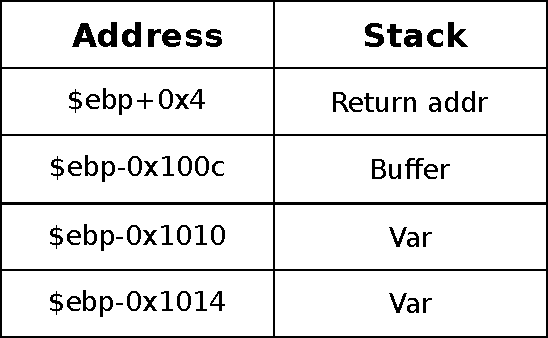
\includegraphics{stack}
  \caption{Stack in the scope of the function \texttt{get\_lines}}
  \label{fig1}
\end{figure}
Thus our attack begins at the offset of $4108$. What the attack does is that we use \texttt{memcpy} to write one byte at a time to \texttt{.data}. The entire exploit can be found in \texttt{doit\_sortfile.py}, but the first part looks like this:
\begin{verbatim}
  exploit  = 'A' * 4108         # Offset
  exploit += '\x50\x84\x04\x08' # memcpy
  exploit += '\xbd\x89\x04\x08' # pop
  exploit += '\x40\xa0\x04\x08' # .data
  exploit += '\x54\x81\x04\x08' # /
  exploit += '\x01\x00\x00\x00' # 1 byte
\end{verbatim}
First we have the offset, then we call \texttt{memcpy} at the given address. The return address we have is a ROP gadget we can use - it pops three times, which are the three arguments given to \texttt{memcpy}. The arguments are the destination (\texttt{.data}), the source (address on a byte we want to use) and the number of bytes (which is 1). This way, we can write one byte at a time to \texttt{.data} (we want to write /bin/sh). When we have what we need, we make a system call:
\begin{verbatim}
  exploit += '\x80\x84\x04\x08' # System
  exploit += '\x84\x94\x04\x08' # Garbage - return
  exploit += '\x40\xa0\x04\x08' # /bin/sh
\end{verbatim}i
First we have the address on the call to \texttt{system}, the following is the return address, which we do not care about (it can be anything). Then finally we have the address on \texttt{.data} where we have /bin/sh. Running \texttt{sortfile} with this exploit will give us a shell, which is exactly what we wanted. \\
The reason we use \texttt{.data} is because it is writable and allocatable, which is a means to work around ASLR and DEP.


\end{document}
